\documentclass{beamer}
\usetheme{DarkConsole}
\usepackage[utf8]{inputenc}
\usepackage[portuguese]{babel}

\title{Julia para Pythonistas}
\author{Melissa Weber Mendonça}
\date{PythonSul 2018}

\begin{document}

\maketitle

\begin{frame}
	\frametitle{Quem é Julia?}
	\begin{center}
		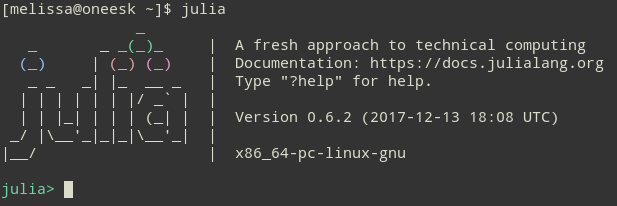
\includegraphics[width=9cm]{juliaconsole.png}
   	\end{center}
	\begin{itemize}
        \item Julia é uma linguagem dinâmica, de alto nível e alto desempenho (disponibilizada em 2012)
   		\item Ideal para computação científica e numérica; também ciência de dados
        \item Bibliotecas adicionais podem ser instaladas via gerenciador de pacotes: \underline{Pkg.add("pacote")}
    \end{itemize}
\end{frame}

\begin{frame}
	\frametitle{Características da linguagem}
    \begin{itemize}
    	\item Free e open source (licença MIT)
    	\item A biblioteca padrão é escrita em Julia
        \item Multiparadigma (quase funcional; baseada em Scheme, MATLAB)
    	\item Tem um compilador sofisticado (JIT/LLVM)
        \item Suporta a computação paralela e distribuída
        \item Permite precisão numérica arbitrária
        \item \emph{Multiple Dispatch}: \underline{tipos} são a chave
    \end{itemize}
\end{frame}

\begin{frame}
	\frametitle{Uma linguagem dinâmica, mas...}
    \begin{itemize}
		\item Código não-vetorizado é rápido
        \item Sistema de tipagem elegante e extensível, com conversão e promoção (o que possibilita o multiple dispatch)
        \item Tipos definidos pelo usuário são tão eficientes quanto os tipos built-in
		\item Possibilidade de chamar funções em C diretamente (sem wrappers ou API's)
		\item Possibilidade de gerenciar outros processos
        \item Macros estilo Lisp e outras possibilidades em metaprogramação
	    \item \emph{Lightweight "green"\ threading (coroutines)}
    \end{itemize}
        \begin{alertblock}{}
    	\begin{center}
			\url{https://julialang.org/benchmarks/}
        \end{center}
    \end{alertblock}
\end{frame}

\begin{frame}
	\frametitle{A hierarquia de tipos}
    
    \begin{center}
    \begin{figure}
		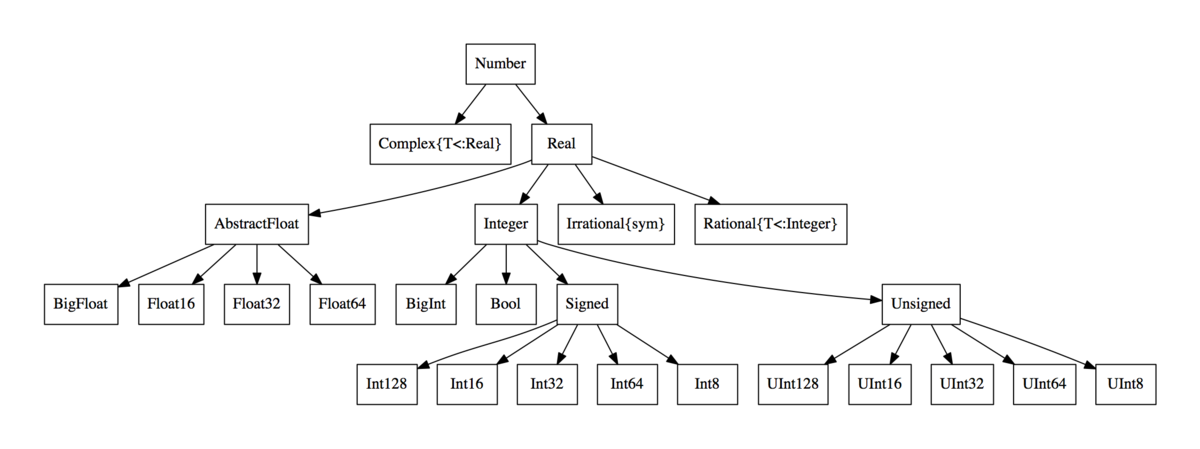
\includegraphics[width=11cm]{Type-hierarchy-for-julia-numbers.png}
        \caption{Hierarquia de tipos numéricos}
    \end{figure}
    \end{center}
    Tipos abstratos servem para definir funções, mas só os tipos concretos (folhas da árvore) podem conter valores.
\end{frame}

\begin{frame}
	\frametitle{"Code Selection"\ vs. OOP\footnote{Veja \cite{juliapaper}}}
	\begin{center}
		\underline{O método é atrelado à função: não ao argumento.}
    \end{center}
    Exemplo: Ao somar duas matrizes A e B, podemos pensar em Python em algo do tipo
    \begin{center}
		 \texttt{A.plus(B)} $\leftarrow $ \emph{single dispatch!}
    \end{center}
    Em Julia, temos
    \begin{center}
    	\texttt{plus(A,B)}
    \end{center}
    A grande diferença é que estamos considerando o tipo de TODOS os argumentos ao escolher a função \underline{plus} correta para ser utilizada com o tipo de argumentos que temos.
%method to be executed in Julia is not chosen by only one argument, which is what
%happens in the case of single dispatch, but through multiple dispatch, which considers
%the types of all the arguments. Julia is not burdened by the encapsulation restric-
%tions (class based methods) of most object oriented languages: The generic functions
%play a more important role than the data types. Some call this type of language
%“verb” based as opposed to most object oriented languages being “noun” based. In
%numerical computing, it is the concept of “solve Ax = b” that often seems to be more
%fundamental, at the highest level, rather than whether the matrix A is full, sparse, or
%structured. Readers familiar with Java might think, “So what? One can easily create
%both examples of code being selected to match the structure of the problem.
%Readers familiar with object oriented paradigms such as C++ or Java are likely
%familiar with the approach of encapsulating methods inside classes. Julia’s more gen-
%eral multiple dispatch mechanism (also known as generic functions, or multi-methods)
%is a paradigm in which methods are defined on combinations of data types (classes).
%Julia has proven that this is remarkably well suited for numerical computing. As an
%aside, in Julia, method ambiguities throw a warning.
%functions have methods!
\end{frame}

\begin{frame}
  \frametitle{Multiple Dispatch}
  Os métodos são definidos de maneira (possivelmente) diferente para cada combinação de argumentos de entrada.
\vfill
  Exemplo:
  \begin{center}
  \begin{minipage}{10cm}
    \texttt{collide\underline{\ }with(x::Asteroid,  y::Asteroid)  = ... }\\
    \texttt{collide\underline{\ }with(x::Asteroid,  y::Spaceship) = ... }\\
    \texttt{collide\underline{\ }with(x::Spaceship, y::Asteroid)  = ... }\\
    \texttt{collide\underline{\ }with(x::Spaceship, y::Spaceship) = ... }
  \end{minipage}
  \end{center}
\end{frame}

\begin{frame}
	\frametitle{Coleções e "A Vingança dos Loops"}
    \begin{itemize}
    \item Julia tem arrays, tuplas, dicionários
    \item "Ah mas os índices começam em 1..."\\ 
    	\begin{center}
	    	\texttt{x = OffsetArray(Float64,  0:9)}
        \end{center}
    \item E a vetorização? Não é necessária pra melhorar o desempenho se já sabemos o tipo de variável que está sendo usada!\footnote{"Users  of  traditional high-level computing languages know that vectorization improves performance. Do most users know exactly why vectorization is so useful?  It is precisely because, by vectorizing, the user has promised the computer that the type of an entire vector of data matches the very first element."\ \cite{juliapaper}}
    \end{itemize}
        
    \begin{center}
    	Pode usar \underline{\texttt{for}} sem medo de ser feliz!
    \end{center}
%Experienced MATLAB users like to say “Life is too short to spend writing for loops.” It is not that “for loops” are inherently slow in themselves. The slowness comes from the fact that in the case of most dynamic languages, the  system does not have access to the types of the variables within a loop. Since programs often spend much of their time doing repeated computations, the slowness of a particular operation due to lack of type information is magnified inside a loop. This leads to users often talking about “slow for loops” or “loop overhead.”

%We see this as the ultimate realization of the famous 1908 quip that Mathematics is the art of giving the same name to different things. by noted mathematician Henri Poincare.
\end{frame}

\begin{frame}
	\frametitle{Metaprogramação}
    Julia tem um sistema de macros, símbolos e \emph{expressions}, que permitem escrever código julia em julia. \\
    \underline{Exemplo:}\footnote{\url{https://stackoverflow.com/questions/23480722/what-is-a-symbol-in-julia}}
    \begin{center}
    \begin{minipage}{8cm}
    	\small{%
	    \texttt{\textcolor{green}{julia>} foo = "hello"}\\
		\texttt{\textcolor{green}{julia>} :foo}\\
		\texttt{:foo}\\
		\texttt{\textcolor{green}{julia>} typeof(:foo)}\\
		\texttt{Symbol}\\
		\texttt{\textcolor{green}{julia>} typeof(foo)}\\
		\texttt{String}\\
		\texttt{\textcolor{green}{julia>} eval(:foo)}\\
		\texttt{"hello"}\\
		\texttt{\textcolor{green}{julia>} eval(foo)}\\
        \texttt{"hello"}\\
        \texttt{\textcolor{green}{julia>} eval("foo")}\\
        \texttt{"foo"}
        }
    \end{minipage}
    \end{center}
	%a macro system that provides custom code generation, providing performance that is otherwise difficult to achieve. A macro is a function that runs at parse time, takes symbolic expressions in, and returns transformed expressions out, which are inserted into the code for later compilation. 

%Macros are necessary because they execute when code is parsed, therefore, macros allow the programmer to generate and include fragments of customized code before the full program is run
\end{frame}

\begin{frame}
	\frametitle{Macros de tradução}
    Permitem ao usuário observar a tradução de um pedaço de código em julia para níveis mais baixos\footnote{\url{https://goo.gl/FUko5L (Stack Overflow)}}:
    \vfill
    %https://stackoverflow.com/questions/43453944/what-is-the-difference-between-code-native-code-typed-and-code-llvm-in-julia}
    \begin{itemize}
		\item \texttt{@code\underline{\ }lowered}
        \item \texttt{@code\underline{\ }typed}
        \item \texttt{@code\underline{\ }llvm}
        \item \texttt{@code\underline{\ }native}
    \end{itemize}
\end{frame}

\begin{frame}
	\frametitle{Não precisa abandonar o Python!}
    Com \texttt{PyCall.jl}, é possível usar Python diretamente dentro do julia:
    \begin{center}	
	    \begin{minipage}{8cm}
			\texttt{\textcolor{green}{julia>} @pyimport scipy.optimize as so}\\
			\texttt{\textcolor{green}{julia>} so.newton(x -> cos(x) - x, 1)}
        \end{minipage}
    \end{center}
\end{frame}

\begin{frame}
	\frametitle{Por que escolher Julia para Data Science?\footnote{\url{http://ucidatascienceinitiative.github.io/IntroToJulia/Html/WhyJulia}}}
    \begin{center}
    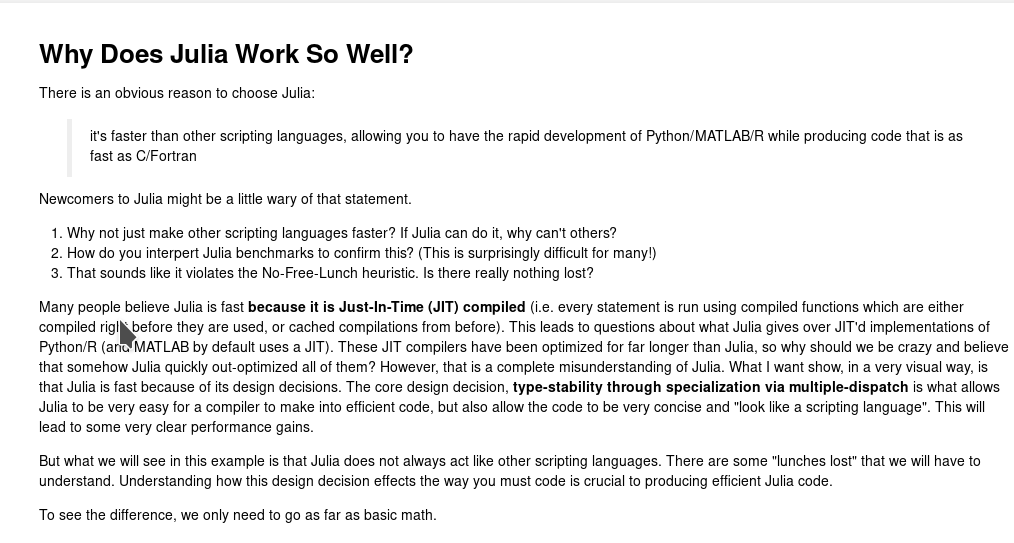
\includegraphics[width=10cm]{whyjulia.png}
    \end{center}
\end{frame}

\begin{frame}
	\frametitle{Tem muito mais pra dizer...}
    \begin{itemize}
    \item Julia é jovem! Muda muito rápido
    \item Documentação ainda está incompleta
    \item Pacotes estão surgindo a todo momento
    \item Só vem $\heartsuit$\only<2>{\footnote{(Fala sério, dá pra chamar uma variável de $\heartsuit$!!!!)}}
    \end{itemize}
\end{frame}

\begin{frame}
	\frametitle{}
    \begin{center}
    	telegram: \texttt{melissawm}\\
        twitter: \texttt{@melissawm}\\
        email: \texttt{melissa.mendonca@ufsc.br}
    \end{center}
\end{frame}

\begin{frame}[allowframebreaks]%in case more than 1 slide needed
  \frametitle{Bibliografia}
    {\footnotesize
    \bibliographystyle{apalike}
    \bibliography{refs}
    }
\end{frame}

\end{document}
